%----------------------------------------------------------------------------------------
%	PACKAGES AND OTHER DOCUMENT CONFIGURATIONS
%----------------------------------------------------------------------------------------
\documentclass[11pt, a4paper,oneside]{ctexbook}

%----------------------------------------------------------------------------------------
%	TITLE PAGE
%----------------------------------------------------------------------------------------

\newcommand*{\titleGP}{\begingroup % Create the command for including the title page in the document
\centering % Center all text
\vspace*{\baselineskip} % White space at the top of the page

\rule{\textwidth}{1.6pt}\vspace*{-\baselineskip}\vspace*{2pt} % Thick horizontal line
\rule{\textwidth}{0.4pt}\\[\baselineskip] % Thin horizontal line

{\LARGE \textbf{国际教育-小学系列} \\[0.3\baselineskip] \textbf{中文版}}\\[0.2\baselineskip] % Title

\rule{\textwidth}{0.4pt}\vspace*{-\baselineskip}\vspace{3.2pt} % Thin horizontal line
\rule{\textwidth}{1.6pt}\\[\baselineskip] % Thick horizontal line

\scshape % Small caps
\href{https://fieldworkeducation.com/about}{Fieldwork-Education}\\[\baselineskip] % Tagline(s) or further description
\href{https://fieldworkeducation.com/curriculums/primary-years}{IPC}\par % Location and year

\vspace*{4\baselineskip} % Whitespace between location/year and editors

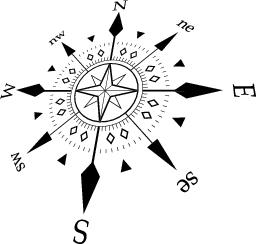
\includegraphics[width=10cm]{compass}


\vfill % Whitespace between editor names and publisher logo

{\itshape2398419426@buaa.edu.cn\par} % Editor list
{\itshape HaotianMichael \par} % Editor affiliation
\vspace*{0.5\baselineskip}
{\scshape 2018} \\ 
{\scshape Powered by \LaTeX \\[0.3\baselineskip]} % Year published

\endgroup}


\usepackage{graphicx} % Required for including pictures
\graphicspath{{Images/}} % Specifies the directory where pictures are stored
\CTEXsetup[format={\Large\bfseries}]{section}    %make section left justifing
%----------------------------------------------------------------------------------------
%       Localization
%----------------------------------------------------------------------------------------
\usepackage[UTF8,adobefonts]{ctex}
\usepackage{array, booktabs}
\usepackage{graphicx}
\usepackage[x11names]{xcolor}
\usepackage{colortbl}
\usepackage{fontspec}
\newcommand{\foo}{\color{baseD}\makebox[0pt]{\textbullet}\hskip-0.5pt\vrule width 1pt\hspace{\labelsep}}

%\setmainfont[Boldont=WenQuanYi Micro Hei]{AR PL SungtiL GB}
%\setsansfont[BoldFont=WenQuanYi Micro Hei]{AR PL KaitiM GB}
%\setmonofont{DejaVu Sans Mono}

%\XeTeXlinebreaklocale "zh"
%\XeTeXlinebreakskip = 0pt plus 1pt minus 0.1pt

\usepackage[top=1in,bottom=1in,left=1.25in,right=1.25in]{geometry}
%\linespread{1.2}

\usepackage[Glenn]{fncychap}

\usepackage{fancyhdr}
\setlength{\headheight}{15.2pt}

%----------------------------------------------------------------------------------------
%       Useful Packages
%----------------------------------------------------------------------------------------
\usepackage{color}
\usepackage{url}
\usepackage[colorlinks, linkcolor=black,anchorcolor=black, citecolor=black]{hyperref}

\usepackage{xcolor} % Required for specifying colors by name
\definecolor{ocre}{RGB}{243,102,25} % Define the orange color used for highlighting throughout the book

% BASE16
\definecolor{base0}{HTML}{181818}
\definecolor{base1}{HTML}{282828}
\definecolor{base2}{HTML}{383838}
\definecolor{base3}{HTML}{585858}
\definecolor{base4}{HTML}{B8B8B8}
\definecolor{base5}{HTML}{D8D8D8}
\definecolor{base6}{HTML}{E8E8E8}
\definecolor{base7}{HTML}{F8F8F8}
\definecolor{base8}{HTML}{AB4642}
\definecolor{base9}{HTML}{DC9656}
\definecolor{baseA}{HTML}{F7CA88}
\definecolor{baseB}{HTML}{A1B56C}
\definecolor{baseC}{HTML}{86C1B9}
\definecolor{baseD}{HTML}{7CAFC2}
\definecolor{baseE}{HTML}{BA8BAF}
\definecolor{baseF}{HTML}{A16946}
\definecolor{Gray}{HTML}{CCCCCC}
\definecolor{linkcolor}{HTML}{EC008C}
\definecolor{codecolorpink}{HTML}{CC00FF}
\definecolor{NoteColorFont}{HTML}{6D727D}
\definecolor{NoteColorLine}{HTML}{C3CAD9}
\definecolor{ExeColorFont}{HTML}{FF9900}
\definecolor{ExeColorLine}{HTML}{FFF678}
\definecolor{ExeColorBack}{HTML}{FFFFCC}
\definecolor{ThinkColorFont}{HTML}{629D81}
\definecolor{ThinkColorLine}{HTML}{93E87D}
\definecolor{ThinkColorBack}{HTML}{C1FA9B}

\usepackage{amsmath,amsfonts,amssymb,amsthm} % For math equations, theorems, symbols, etc
\usepackage{booktabs} % For tables
\usepackage{tabularx}
\usepackage{multirow} % for multiple row tables.
\usepackage{lettrine}    %expand font size 
\usepackage{indentfirst}  %indent at beginning


%\makeatletter
%\renewcommand{\section}{\@startsection{section}{1}{0mm}
%  {-\baselineskip}{0.5\baselineskip}{\bf\leftline}}
%\makeatother


%----------------------------------------------------------------------------------------
%       Some Extra Definitions
%----------------------------------------------------------------------------------------

\RequirePackage[framemethod=default]{mdframed} % Required for creating the theorem, definition, exercise and corollary boxes

% Exercise box
\newmdenv[skipabove=10pt,
skipbelow=10pt,
rightline=false,
leftline=true,
topline=false,
bottomline=false,
backgroundcolor=ExeColorBack,
linecolor=ExeColorLine,
innerleftmargin=5pt,
innerrightmargin=5pt,
innertopmargin=5pt,
innerbottommargin=5pt,
leftmargin=0cm,
rightmargin=0cm,
linewidth=12pt]{eBox}

% Thinking box
\newmdenv[skipabove=10pt,
skipbelow=10pt,
rightline=false,
leftline=true,
topline=false,
bottomline=false,
backgroundcolor=ThinkColorBack!30,
linecolor=ThinkColorLine,
innerleftmargin=5pt,
innerrightmargin=5pt,
innertopmargin=5pt,
innerbottommargin=5pt,
leftmargin=0cm,
rightmargin=0cm,
linewidth=12pt]{tBox}

% Note box
\newmdenv[skipabove=10pt,
skipbelow=10pt,
rightline=false,
leftline=true,
topline=false,
bottomline=false,
backgroundcolor=NoteColorLine!15,
linecolor=NoteColorLine,
innerleftmargin=5pt,
innerrightmargin=5pt,
innertopmargin=5pt,
innerbottommargin=5pt,
leftmargin=0cm,
rightmargin=0cm,
linewidth=12pt]{nBox}

% Boxed/framed environments
\newtheoremstyle{ocrenumbox}% % Theorem style name
{0pt}% Space above
{0pt}% Space below
{\normalfont}% % Body font
{}% Indent amount
{\small\bf\sffamily\color{ExeColorFont}}% % Theorem head font
{\;}% Punctuation after theorem head
{0.25em}% Space after theorem head	
{\small\sffamily\color{ExeColorFont}\thmname{#1}\nobreakspace\thmnumber{#2}% Theorem text (e.g. Exercise 2.1)
\thmnote{\nobreakspace\the\thm@notefont\sffamily\bfseries\color{black}---\nobreakspace#3.}} % Optional theorem note
\renewcommand{\qedsymbol}{$\blacksquare$}% Optional qed square

\newtheoremstyle{purplenumbox}% % Theorem style name
{0pt}% Space above
{0pt}% Space below
{\normalfont}% % Body font
{}% Indent amount
{\small\bf\sffamily\color{ThinkColorFont}}% % Theorem head font
{\;}% Punctuation after theorem head
{0.25em}% Space after theorem head	
{\small\sffamily\color{ThinkColorFont}\thmname{#1}\nobreakspace\thmnumber{#2}
% Theorem text (e.g. Thinking 2.1)
\thmnote{\nobreakspace\the\thm@notefont\sffamily\bfseries\color{black}---\nobreakspace#3.}} % Optional theorem note
\renewcommand{\qedsymbol}{$\blacksquare$}% Optional qed square

\newtheoremstyle{blackbox} % Theorem style name
{0pt}% Space above
{0pt}% Space below
{\normalfont}% Body font
{}% Indent amount
{\small\bf\sffamily}% Theorem head font
{\;}% Punctuation after theorem head
{0.25em}% Space after theorem head
{\small\sffamily\color{NoteColorFont}\thmname{#1}\nobreakspace\thmnumber{#2}
% Theorem text (e.g. Theorem 2.1)
\thmnote{\nobreakspace\the\thm@notefont\sffamily\bfseries---\nobreakspace#3.}}% Optional theorem note

% Defines the theorem text style for each type of theorem to one of the three styles above
\theoremstyle{ocrenumbox}
\newtheorem{exerciseT}{Exercise}[chapter]
\theoremstyle{purplenumbox}
\newtheorem{thinkingT}{Thinking}[chapter]
\theoremstyle{blackbox}
\newtheorem{noteT}{Note}[section]

\newenvironment{exercise}{\begin{eBox}\begin{exerciseT}}{\hfill{\color{ExeColorFont}\tiny\ensuremath{\blacksquare}}\end{exerciseT}\end{eBox}}
\newenvironment{thinking}{\begin{tBox}\begin{thinkingT}}{\hfill{\color{ThinkColorFont}\tiny\ensuremath{\blacksquare}}\end{thinkingT}\end{tBox}}
\newenvironment{note}{\begin{nBox}\begin{noteT}}{\end{noteT}\end{nBox}}

%----------------------------------------------------------------------------------------
%       Code Environment
%----------------------------------------------------------------------------------------
\usepackage{minted}
\usemintedstyle{manni}

% code box
\newmdenv[backgroundcolor=base7,
linecolor=baseD,
bottomline=false,
leftline=true,
rightline=false,
topline=false,
linewidth=2pt,
leftmargin=13pt]{pcodeBox}

\renewcommand{\theFancyVerbLine}{
  \sffamily
  \textcolor{baseB}{\arabic{FancyVerbLine}
  }
}

\usepackage{caption}

%\captionsetup{type=codeCaption}
\newenvironment{codeBox}{\begin{pcodeBox}\fontsize{9pt}{9pt}}{\end{pcodeBox}}
\newenvironment{codeBoxWithCaption}[1]{\begin{pcodeBox}[frametitle={\captionof{listing}{#1}\color{base6}\rule{\textwidth}{0.7pt}}]\fontsize{9pt}{9pt}}{\end{pcodeBox}}

\BeforeBeginEnvironment{minted}{\begin{codeBox}}
\AfterEndEnvironment{minted}{\end{codeBox}}

%----------------------------------------------------------------------------------------
%       Lists
%----------------------------------------------------------------------------------------
\usepackage{enumitem}
\setlist[description]{labelindent=22pt} 

%----------------------------------------------------------------------------------------
%       Main Body
%----------------------------------------------------------------------------------------
\begin{document}

\pagestyle{empty} % Removes page numbers
\titleGP % This command includes the title page

\frontmatter
\pagestyle{plain}
%\chapter{译者序}


\subsection{关于FIELDWORK-EDUCATION}
     \lettrine[lines=1]{F}{IELDWORK-EDUCATION}本身是一家为学校提供专业、适用和实时的国际化教育机构\footnote{在标题页有该网站链接},创立于1984年。该机构目前有为学校提供学前、小学、中学的国际课程。\par

\subsection{关于IPC}
     \lettrine[lines=2]{I}{PC}全称International Primary Curriculum。国际小学课程,是FIELDWORK-EDUCATION为小学生提供的课程。主要受众是5-11岁的小学生。\par

\subsection{关于本次翻译}
     \lettrine[lines=2]{本}{次翻译工作}我们将每一单元的翻译作为一个Project,每一个项目分为排版和翻译工作两部分,排版使用\LaTeXe,翻译为人工翻译。全书按照原版的目录索引以章节作为单位进行翻译。每一个项目的源代码和源文件都作为模板托管在\href{https://gitlab.com/haotianmichael/LatexTemplate}{GitLab}上。\par
     
     


    

\frontmatter
\tableofcontents


\mainmatter
\pagestyle{fancy}
\chapter{基本信息}
    这一部分详细介绍了本单元学习的时间分配,和其他课程的联系以及教学目标的评价。

\section{时间分配}
    本单元的学习预计会持续大约3周的时间。
    下面的时间分配表仅仅作为参考,具体细节和每一个学校自己的教学计划和内容有关。


\begin{table}[h]     
\begin{tabular}{l|l|l}
\hline
\colorbox[gray]{0.95}{ & 小时数 & 周数 } \\
\hline
学习入口、获取知识、主题阐述 &  4 & 1\textbackslash2 \\
灵感单元的学习  & 16  &   2  \\
学习出口  & 4  &  1\textbackslash2 \\
\hline
\end{tabular}
\end{table}



\section{和其他IPC课程的联系}
    本单元课程的学习并没有突出什么主题,因此是独立于其他IPC课程目标存在的。下面是本单元独立于其他主题的教学目标。
    孩子们将会:
    \begin{itemize}
      \item 了解到最新的关于大脑和学习的一些研究和资料 
      \item 掌握自己的行为是如何影响自身的学习效果的
      \item 能够将所学到的理论知识运用到自己的学习中并思考这样做的结果
    \end{itemize}


\chapter{学习目标}


\section{脑波单元的学习目标}
\footnote{这里和1.2部分重复}孩子们将会:
      \begin{itemize}
        \item 了解到最新的关于大脑和学习的一些研究和资料 
        \item 知道大脑的组成部分及其功能
        \item 了解学习的不同方式  
        \item 了解一些如何提高学习技巧和学习态度的知识
        \item 了解在学习过程中合作和全球化意识的重要性
      \end{itemize}  
 

\chapter{学习评估}
    您的孩子每天是不是把几乎所有的时间都花在学习上?\par
    当学习完这个主题单元\footnote{指灵感-单元}的内容之后,我们希望在以后每一个单元的学习过程中都能够回答这样一个问题————我们的孩子在学习能力上有哪些提高? \par
    我们总结了关于学习能力三个需要思考的领域和三种需要评价的学习类型。 \par

\section{三个领域:学术、私人和国际}
    这三个领域分别为:学术圈、私人领域和国际化的场景。要完成对这三个领域的思考,你需要访问IPC关于每一个主题的学习目标(包括国际化的内容)和IPC课程的个人目标————该列表可以在\href{https://members.greatlearning.com/ipc/documents?category=31}{IPC实施文件}的附录A中找到。当然你也可以在会员区的\href{https://members.greatlearning.com/ipc/assess/learninggoals}{评估部分}找到IPC学习目标比较完整的版本。


\section{三种类型:知识、技能和理解}
    这三种类型包括知识、技能和理解。我们相信区分这三者对孩子学习的发展至关重要。我们还认为知识、技能和理解力三者都有其独特的特征,这些特征会影响每一个人的计划、学习、教学、评估和报告方式。从这个角度看,这些特征之间的不同含义影响是深远的,并值得进一步的思考。


\subsection{知识}
    \textbf{知识}指的是真实的信息。尽管要回忆起这些知识并不是简单事,但相对来说知识本身是比较容易能够传授和评估的(通过智力测试、课堂测试、单项选择等)。你可以要求孩子们去研读需要学习的知识,但是你也应该告诉他们那些他们需要知道的知识。知识本身是不断更新迭代的,这对于学校来说是一个挑战,因为学校必须能够选择在特定的一段时间内适合孩子们了解和学习的知识。 \par
    IPC\footnote{国际小学课程}并不提供知识评估(测试或者考试)的例子,因为IPC课程中的知识内容可以适应任何国家课程的要求。


\subsection{技能}
    \textbf{技能}指的是那些孩子们能够做的事情。技能需要在实践中学习并需要时间去掌握。技能的特点是你训练的时间越长,那这项技能你掌握的越熟练。技能也是可以传授的,往往比知识更稳定————这几乎适用于所有学校的教学科目。\par
    IPC通过\href{https://members.greatlearning.com/ipc/assess/}{IPC学习计划评估}支持学习追踪和学习评估,该计划评估的内容包括老师的评估准则、学生的评估准则和学习建议。

\subsection{理解}
    \textbf{理解}指的是对一些概念思想的逐渐把握和发展,换句话讲就是我们经常说的“灵光一现”的时刻。人的理解是不断发展的。  \par
    IPC并不能为您的孩子们评估理解力。但是课程允许您提供一整套不同的体验机制来加深孩子们的理解力。\par
    \begin{note}
      请注意: \par
      和IPC学习计划评估一样,我们还和Classroom Monitor\footnote{一家在线学习评估机构}合作推出了一套线上评估跟踪工具。关于如何注册并使用这套工具,请给\underline{member@fieldworkeducation.com}写信询问详细的信息。
    \end{note}


\section{规划评估}
     一旦你开始为各个IPC课程主题规划不同的学习目标,那在每一个单元的学习过程对评估目标进行规划也就变的很重要了。评估需要面面俱到但是也需要每一个都严格以确保孩子们学到了我们学习规划中的所有内容。下面的图表提供的一套机制或许可以帮助实现这一点。


\section{帮助孩子们自己评估自己的学习}
     除了教师的评估之外,让孩子们自己参与整个评估过程并据此设定下一步的提高方案也是至关重要的。让孩子们对每一个单元的学习做出自我评估(使用学生评估准则来评价技能,使用学校提供的其他方式来评估知识和理解力)。  \par
     他们可以使用下面的标题来列出新学习的知识,技能和理解。
     \begin{itemize}
       \item 我现在知道的新事物
       \item 我现在可以做的新事情
       \item 我现在开始理解的新概念
     \end{itemize}   \par
     从学习过程中的不同角度和方面记录孩子们对自己的评估:
     \begin{itemize}
       \item 哪一方面做得比较好?
       \item 哪些方面是下次有机会提高的,方法是什么?
       \item 哪些方面是最最有趣的? 
       \item 更喜欢如何学习——独自,两个人,小组,人多一些的组还是整个班级?
       \item 更喜欢哪一种学习和记录的方式——记笔记、讨论还是动手实践?这项评估也可以支持IPC课程中的个人目标发展。
     \end{itemize}  \par
    

\section{更多信息}
     想要了解到更多的关于知识、技能和理解评估的信息,请访问:
     \begin{itemize}
       \item  \href{https://members.greatlearning.com/ipc/documents?category=31}{IPC实施档案}
       \item  \href{https://members.greatlearning.com/ipc/assess/aflfile}{学习评估实施档案}
       \item  \href{https://members.greatlearning.com/ipc/bottomline9/}{IPC自我反省程式}
     \end{itemize}  
     \par
     或者直接联系团队:\underline{member@fieldworkeducation.com}

\chapter{学习入口}
    让同学们想一些自己比较擅长的事情。完全可以是课堂之外的事情。如果有同学提到了比如艺术、体育、音乐、电脑游戏这些外延比较宽泛的领域,让他们描述的更清楚一些。因为可能需要他们将自己的技能和知识教给别人。\par
    给每一个同学一张卡片,每一位同学可以在上面写上他们的名字和他们能够教给别人的东西比如:"40米开外的铅球扔法"、“站在别人的头上”、“同时玩4个球”、“如何同时快速得出两个数的乘积“……或许同学们的想法会更加奇特和有意思,老师在筛选的时候需要保证最基本的安全。\par
    告诉同学们他们即将成为别人的老师,将自己的高超技术传授给别人。将同学两人分组,这样每一位同学既是老师又是同学。例如,老师可以从帽子中抽出卡片,将它们显示在墙上并邀请同学们随机选择。\par
    首先留时间给同学去思考他们已经学习过的关于快速学习和快速教学的知识,然后收集每个人的观点,以这些为基础来规划教学。可以从这几个方面作出提示:\par
    \begin{item}
      \item 和教学内容相关的知识、技巧和理解。应该如何具体辨别和掌握?
      \item 老师的各种教学方法————老师会给学生提供什么阅读材料(比如帮助手册)、提供什么示范(建模)、会有什么具体的课堂展示(比如PPT)或者以上三者都有?
      \item 对学习者有利的事情————他们使用的语言、如何调整出他们的积极心态?这些和我们已经学过的关于学习的知识有什么联系?
      \item  学习评估————学习者如何知道他们是否进步?我们如何监督他们的进度并根据实际情况提供帮助?学成的标准具体会是什么?\footnote{这也是任务的一部分,学生们必须得自行设计自己的评估准则。不过学生可以参考他们已经很熟悉的IPC学习计划评估。如果学校并没有使用这套计划,那学生可以考虑自行简化和修改学校的学习评估系统。IPC评估准则一共有三个阶段:初学、一般和精通。希望这些可以帮助学生自行设计出自己的评估准则。(IPC准则可以再哎会员区下载)} 
    \end{item}
    \par
    固定时间让学生们设计和准备他们即将需要教授的内容。并且需要考虑到他们上课时候需要用到的道具。\par
    老师需要将学习入口上课时间划分为两部分。这样第一部分结束之后学生还可以有足够的时间去准备和配备他们上课需要的装备、材料和教学资源。他们的学习过程和教学过程也会非常顺利。\par
    一旦学生准备好,两人分组开始第一部分:\par
    给同学们最多1小时时间来实施完成第一部分的教学和学习。然后两人身份交换,老师成为学生;学生成为老师。给另外一小时进行第二部分的学习和教学。在每一部分的过程中鼓励孩子们互相监督和评价学习进度——在每部分结束的时候,给双方一次机会一起完美结束。\par
    同学可能会使用自己的视角来进行监督。如果你正在使用IPC学习计划评估,那么三个阶段(初学、一般、精通)可以比做成一座高山,到达山顶就是精通。又可以看成是还在生长的大树。老师们甚至可以做一个全班同学共同的监督工具。每一位同学可以将自己的图片放到相应的阶段上。每一个人都应该确保学习并不是竞争,每一次评估将会是一次帮助我们了解我们的学习过程,我们还可以上升的领域、我们需要提高的部分的一次机会。\par
    全班一起讨论过程中到底发生了什么?你或许想画一张思维导图来记录这一切比如:\par
    \begin{item}
      \item 学习起来很容易因为……
      \item 学习起来很吃力因为……
      \item 教起来很容易因为……
      \item 教起来很吃力因为……
    \end{item} 
    问同学,如果他们即将有另一次机会来做一遍。他们希望哪里被改善来提高教学效果。\par
    学习入口的结束应该是做出一个”如何成为一个更好的老师的标准“或者”如何成为一个更好的学生准则”。然后将这两份报告贴在展示区,在接下来的一年内都可作为参考。\par
    学生们应该对学习入口的内容非常了解。但是如果你的学生是新来的,对IPC不是很了解,老师需要复习一下相关内容。每一个IPC学习主题都会有一个学习入口,学习入口的目的主要是让学习者对即将学习的主题提起兴趣,并且有一些这方面的思考。老师可以问一下学生们学习入口到底对自身的学习过程有什么正面作用,甚至有什么进一步的帮助。\par
    
    

\chapter{知识获取}
    

\chapter{全局观}
    如果巧克力种在树上那岂不是很有意思?嗯,当然很有意思。但是如果我说,我们打算去自己制作一些巧克力的话,是不是也很有意思?对!我们打算自己制作一些巧克力。而且我们还要探索关于巧克力更有趣的事情……


\include{chapter/7-ExplainingTheThem}
\chapter{知识图谱}
   


\section{可可}
     可可发源于玛雅文明,主要生长在危地马拉。是一种价值很高的商品。在加工之后,可可树上的豆子会被制作为巧克力饮品中的巧克力。想我们一样,玛雅人也喜欢巧克力,不过不同的是我们将巧克力做成巧克力棒来吃,而玛雅人是喝!他们用辣椒等香料调味巧克力饮料,有时他们会用蜂蜜。他们确保自己的音频会有很多的泡沫,我们在很多地方看到这种描述。我们也看到过一些关于玛雅人如何制作者写又泡沫的饮品————将液体从高处倒进另一个容器中。可可豆在烘烤之后,便于存储和运输。也正在因为这个原因,可可在后经济学和接触时期的巨大市场经济中成为一种很重要的交换媒介(货币)。从这个角度来讲,玛雅人实际上是在喝钱!\par
     将可可作为一种货币和饮品的传统被由中美洲和南美洲的阿兹特克人延续下来。这帮人将这种饮品成为“chocolatl”\footnote{巧克力的英文是chocolate}。该饮品被作为“神的食物”并放在金被子中作为皇家贡品。据说皇帝蒙特祖玛一天要喝50杯!可可不仅是一种很招人喜爱的饮品。更是玛雅人和阿兹特克人宗教活动和社会活动中很重要的组成部分。\par

\section{哥伦布和科尔特斯}
     16世纪的探险家哥伦布,在1504年的时候,从当时的新世界————就是现在的美洲带了一些可可回到西班牙。西班牙国王和皇后并没有认识到哥伦布带回来的这些豆子的重要性,他们倒是很看重哥伦布带回来的黄金和奇珍异宝。豆子的重要性被1519年的探险家科尔斯特发现了。刚开始蒙特祖玛国王赠予很多的可可豆,但科尔斯特并不喜欢。直到他发现这些豆子可以被作为当地的货币使用的时候(4个豆子换一只兔子,10个豆子换一个奴隶),这时候他才意识到这一发现的重要性————他可以在树上种出钱来。

\section{关于埃尔南 科尔斯特的更多信息}
     科尔斯特是一位西班牙的探险家,他在1521年的时候征服了阿兹克特王朝。科尔斯特利用自己洁白的皮肤和小胡子让蒙特祖玛二世国王相信自己就是神。上古的预言成真了。而且国王也相信了这件事情。但是之后科尔斯特并没有表现的像一个神一样。他们被驱逐出境。但是科尔斯特不久之后又回来了,这次他带了600名士兵。他捉住了蒙特祖玛二世国王并毁掉了阿兹特克王朝的首都特诺奇蒂特兰城。并在废墟上建立了墨西哥城。原始城市的所有遗迹都是主殿的废墟。


\section{巧克力酱}
     从韦拉克鲁斯到塞维利亚的巧克力官方装箱发生在1585年。在17世纪的欧洲贵族中,辣椒被替换成为糖从而变得更加流行了。英国人,法国人和德国人将这些可可引进到自己的殖民地。在美国,巧克力是在马萨诸塞州多切斯特首次制作的。第一个巧克力棒是由弗莱在1847年在伦敦制作的。两年后,吉百利制作了类似的产品。 牛奶巧克力是由Daniel Peter于1876年在瑞士制造的,只需加入奶粉即可。第一次世界大战后几年,雀巢推出了白巧克力。它含有可可脂,但根本没有可可固体。 出于这个原因,有些人认为它不应该被称为“巧克力”。今天,世界上80%的巧克力仅由六家跨国公司生产,包括雀巢,火星和吉百利。最大的巧克力消费者是瑞士,每人每年消费超过10公斤(22磅)。 排名前十位的消费者包括:瑞士,德国,奥地利,爱尔兰,英国,挪威,爱沙尼亚,斯洛伐克,瑞典和哈萨克斯坦。


\section{主打产品}
      




\section{热带生物群系}



\section{可可树}


\section{收获}



\section{}

\chapter{地理单元的学习目标}
    同学将会:\par

    \begin{itemize}
      \item 了解特定的地区是如何被人类行为干涉的
      \item 了解特定自然地区对人类的生活是如何影响的
      \item 了解自己的住宿国家的天气条件和气候条件,思考这些条件是如何影响环境和当地人的生活的
      \item 能够明白地理的专业术语
      \item 能够使用不同层面的地图进行一些特定地理特征和位置的定位和识别
      \item 能够通过第二信息源来获得地理信息
      \item 能够就一些自然环境的特征给出自己的建议和看法,并能够谈谈这些地区的环境的优化措施
      \item 能够谈一些地理方面的知识和理解,回答关于地理和环境特征的问题
      \item 理解小地区是如何适应更大的地理版图的
      \item 理解到:自然环境可以被破坏,但是也可以被优化
    \end{itemize}  

\chapter{地理任务-1}



\section{学习目标}
    \begin{itemize}
      \item 了解居住国家的天气和气候条件,以及这些条件是如何影响当地环境和当地人们的生活的。
      \item 能够使用地理专业术语
      \item 能够使用不同层面的地图来对一些特定的地理位置进行定位
      \item 能够通过第二信息员获得地理信息
      \item 能够谈论一些关于地理方面的知识,和 回答一些关于自然条件和地理特征方面的问题
      \item 理解小地区是如何适应比较大的地理版图的
    \end{itemize}  


\section{探究活动}
     巧克力是怎么做出来的?\par
     一些孩子们会记住巧克力是从树上长出来的(复习知识获取单元的知识)。在白板上画一张图片
     A chocolate is not that simple as you thought.
     


\section{记录活动}
   


\section{个人目标}

\chapter{地理任务-2}

\section{学习目标}
    \begin{itemize}
      \item 了解特定地区的性质是如何影响当地人们的生活的。
      \item 能够使用地理专业的术语
      \item 能够使用二级信息源获取地理信息
      \item 能够交谈关于地理的话题并且理解和回答一些关于地理相关的问题
      \item 了解小地域是如何适应比较大的地理版图的
    \end{itemize}  

\section{探究活动}
   你想要在一个种满可可树的农场里工作吗?你会吃很多的巧克力吗?让我们一起探究一下。\par
   从解释“经济作物”这个单词开始:就是这些产品被种不是用来当地消费的,而是赚钱用的。所以说那些中可可树的人是不会吃巧克力的!\par
   他们为什么不吃巧克力呢?邀请同学提出建议(巧克力会在热天气下融化,而且这些东西都很贵)。农场主将可可豆卖到其他的国家比如美国,瑞士,德国和比利时。这些国家(工业化程度更高和更加有钱的)负责加工和将这些可可豆量产化为巧克力。\par
   \begin{itemize}
     \item Cacao——树的名字
     \item Cocoa——种子里面的豆
     \item Cocoa exports——那些卖可可豆的国家(供应商) 
     \item Cocoa importers——那些买可可豆的国家(加工商)
   \end{itemize}   
   下面的一些网址会提供一些有用的链接和信息:\par
   \begin{itemize}
     \item \href{http://globaldimension.org.uk/news/item/14702}{globaldimension.com}Global Dimension提供探索巧克力生产全球方面的信息和视频。
     \item \href{http://www.sfu.ca/geog351fall03/groups-webpages/gp8/intro/intro.html}{geog351fall03.com}- 世界巧克力地图集探索巧克力生产和消费的地理位置。
     \item \href{http://ngm.nationalgeographic.com/ngm/0404/resources_geo2.html}{nationalgeographic.com}国家地理网站提供了有用的背景信息:巧克力之路(附带链接)。
   \end{itemize}
   高年级的孩子们可以探究下面的问题:\par
   \begin{itemize}
     \item 当地的人通过种植可可豆转到的利益往往很少
     \item 一些农场主甚至雇用童工,都是一些想通过打工来帮助自己的家庭度过困难的苦孩子。
   \end{itemize}  
   

\section{记录活动}
     请同学在普通的世界轮廓地图上定位一些巧克力的加工商所在国家。并在这些国家的边上标上名字(美国,英国,瑞士,德国,比利时等)。\par
     现在将两张地图放到一起————在任务1中做的可可豆的供应商所在的国家和这次任务中做的可可豆的加工商所在的国家。现在同学们可以很清楚的看见巧克力的供应商和加工商。将供应商和加工商之间的出口画上一条线,并用颜色分清供应商和加工商。\par
     高年级的同学能不能想出一个办法来解决低收入和童工的方法?如何才能使得他们的建议得到实施?老师也可以鼓励孩子们写信给一些主要的巧克力加工商问一问他们是如何处理这些事情的?或者参考国际化任务1。\par
     技术链接: 探究可可树是如何生长的,以及他们的加工流程和可可豆制作成为巧克力的流程。将这些步骤做成一个插图形式或者卡通动画。\par
     下面的网址可以提供一些有用的帮助:\par
     \begin{itemize}
        \item \href{http://www.dubble.co.uk/bean2bar}{dubble.com}Dubble网站为儿童提供信息和视频.
        \item \href{http://www.divinechocolate.com/uk/about-us/research-resources/divine-story/bean-to-bar}{divinechocolate.com}Divine Chocolate提供信息和照片,介绍从可可树到消费者的巧克力制作过程。
        \item \href{http://www.scharffenberger.com/our-story/artisan-process/}{scharffenberger.com}Scharffenberger网站解释了他们工厂生产巧克力的过程。
        \item \href{cocoaskiss.blogspot.com }{cocoaskiss.com} - Cocoaskiss网站为教师提供有关巧克力的所有信息和照片。
     \end{itemize}  
     


\section{个人目标}
    \begin{itemize}
      \item 沟通
      \item 探究
      \item 道德
      \item 深思  
    \end{itemize}  
   

\chapter{地理扩展任务}


\section{学习目标}
    \begin{itemize}
      \item 了解特定的地域是如何影响人类的行为的
      \item 了解特定地域的性质是如何影响人类的生活的
      \item 能够使用地理的专业术语
      \item 能够通过二级信息获取地理信息
      \item 能够清晰的表述关于一片自然环境的特征,以及如何对其进行改善。
      \item 能够谈论关于地理相关的话题,可以理解并回答一些关于地理的问题。
      \item 理解小地区是如何适应比较大的地理版图的
      \item 理解自然环境可以被破坏,当然也可以被修复。
    \end{itemize}  

    

\section{扩展任务}
     咖啡和巧克力有什么相同点?它们生长在相同的气候条件,也同样都是经济作物。\par
     "长在树上的钱"。像同学们介绍这句谚语。并适当的谈论一下关于经济作物的事情比如咖啡和可可豆。大面积的热带雨林被砍伐用例作为经济作物的产地。这种行为会不会对自然环境和当地的居民造成什么影响?\par
     下面的网站提供了一个很好的出发点:\par
     \begin{itemize}
       \item  \href{http://environment.nationalgeographic.com/environment/photos/rainforest-deforestation//%23/madagascar-slash-burn_278_600x450.jpg}{pictures.jpg}国家地理网站上有雨林砍伐森林的照片。
       \item  \href{http://www.rainforestsaver.org/what-slash-and-burn-farming}{rainforest.com}Rainforest Saver网站解释了什么是刀耕火种。
       \item  \href{http://www.edenproject.com/rainforest/}{edenproject.com}伊甸园项目网站解释了雨林的重要性。
       \item  \href{http://www.worldcocoafoundation.org}{worldcocoafoundatio.com}世界可可基金会网站提供有关可持续可可种植的信息和视频。
     \end{itemize}  
     
     同学可以小组内讨论并探究这些问题:\par
     \begin{itemize}
       \item '刀耕火种'——这些事情是在哪里,因为什么发生的?
       \item ’经济作物‘——经济作物的利弊?
       \item ‘森林砍伐’——这种行为会对地球的气候,植被和动物造成什么样的影响?
       \item ‘保守估计在2050年会有不到5\%的热带雨林留下来’——为什么我们需要拯救世界的热带雨林。
       \item ‘人类’——当地人还可以以什么为生?
     \end{itemize}  
     你可以根据每一个小组的能力不同,分配不同的工作给他们。\par
     同学可以通过话剧,诗歌或者歌曲的形式来展示自己的成果。最后全班一起讨论大肆破坏热带雨林种植经济作物的利弊是什么?\par
     下面的视频解释了可可树的有机种植如何拯救热带雨林:\par
     \begin{itemize}
       \item \href{http://video.nationalgeographic.com/video/player/news/environment-news/domrep-cacao-wcvin.html}{youtube.com}国家地理网站上有关于可可有机农业如何实际拯救多米尼加共和国热带雨林的视频。
     \end{itemize}  
     
     

     
\section{个人目标}
    \begin{itemize}
      \item 沟通
      \item 探究
      \item 道德
      \item 尊重
      \item 深思
    \end{itemize}  


\chapter{历史单元的学习目标}
    同学们将会:\par
    \begin{itemize}
      \item 通过研究了解到一些关于古时代的主要大事件、纪时和历史人物。
      \item 了解在某个特定时期人们的生活。
      \item 通过研究了解不同时代的人类生活的相似点和不同点。
      \item 能够给出一些特定事件的具体原因和转折点及其原因。
      \item 能够从简单的来源收集信息。
      \item 能够使用自己所学的知识和理解对过去做出合理的解释。
    \end{itemize}  


    

\chapter{历史单元任务-1}

\section{学习目标}
     \begin{itemize}
       \item 通过研究了解到一些关于古时代的主要大事件、纪时和历史人物。
       \item 了解早某个特定时期人们的生活。 
       \item 能够给出一些特定时间的具体原因和转折点及其原因。
       \item 能够从简单的来源收集信息。
       \item 能够使用自己所学的知识和理解对过去做出合理的解释。
     \end{itemize}  


\section{探究活动}
   人类喝巧克力的历史已经有上千年的了————不是那种在超级市场见到的“热巧克力”,而是一些叫做“xocolatl”或者“chocolatl”的东西。\par
   问一下同学,以小组为单位探究巧克力的历史,下面是主要需要关注的问题:\par
   \begin{itemize}
      \item 什么是“chocolatl”?谁制作了它?是如何做的?
      \item 谁第一次喝,当时的情况是怎么样的?
      \item 它和我们现在喝的巧克力有什么不一样?
      \item 哥伦布第一次将可可豆带回到西班牙的时候,可可豆为什么被忽视了?
      \item 哪一位西班牙的探险家第一次大面积种植和栽培可可豆呢?  
      \item 之后又发生了什么?
   \end{itemize}  

   下面的书籍和网址提供了相应的帮助:\par
   \begin{itemize}
     \item The Story of Chocolate, by Caryn Jenner, Dorling Kindersley, 2005
     \item The Story of Chocolate, by Katie Daynes, Usborne Publishing, 2006
     \item \href{http://mexicolore.co.uk/maya/chocolate/}{mexicolore.com}- 这个教育网站专门关注巧克力(可可)在阿兹特克人和玛雅人中的作用,文章适用为老师和孩子们。
     \item \href{http://www.exploratorium.edu/exploring/exploring_chocolate/choc_2.html}{exploratorium.com}Exploratorium网站探索巧克力的历史。
     \item \href{http://www.inventors.about.com/od/foodrelatedinventions/a/chocolate.htm}{inventors.com}- About.com网站有可可豆的历史时间表。 
     \item \href{http://www.thestoryofchocolate.com}{thestoryofchocolate.com}“巧克力的故事”中有一个“谁依赖它?”部分,其中包含有关巧克力对过去人们的影响的信息
     \item \href{http://www.sfu.ca/geog351fall03/groups-webpages/gp8/history/history.html}{sfu.ca.com}SFU网站包含有关巧克力历史的有用信息。
   \end{itemize}  
   

\section{记录活动}
     以小组为单位,请孩子们利用自己探究的成果写一系列短话剧和小插曲,通过这种形式来表现巧克力的发展历史。比如:   \par

     \begin{itemize}
       \item  从阿兹特克国王蒙特祖玛开始,情景就是为自己的客人在提供放在金杯中的可可豆。
       \item  哥伦布向西班牙的国王和王后展示了珠宝、金银和大量的可可豆,但是国王和王后对可可豆视而不见。
       \item  这时候科尔特斯上场,他不喜欢喝可可豆煮的饮料,但是他发现可可豆竟然被用来作为货币使用!
       \item  科尔斯特回到西班牙之后,带回了可可豆。这时候,西班牙人在饮料中添加了白糖而不是香料,一夜之间所有人都爱上了巧克力!
       \item  但是不是所有的人都负担得起和巧克力的费用。只有欧洲的王室贵族,富人和国王才能享受这种殊荣。
     \end{itemize}  

     等等。\par
     最后,同学们应该画出一幅有插图的时间轴,这幅画上带有每一个当事人的名字和事件发生的时间。这些事件需要从蒙特妈祖引出可可豆开始记录一直到今天我们用钱买巧克力。\par
     艺术链接:研究阿兹特克艺术。 用一个饮用杯形状的粘土做一个简单的捏锅或线圈罐。 烘烤,装饰和上釉。 使用黄色作为基础,并用黑色,棕色和白色几何图案装饰。 然后在烘烤。\par
     下面的网址提供了一个比较好的出发点。\par
     \begin{itemize}
       \item \href{kinderart.com/sculpture/clay.shtml }{kinderart.com}Kinderart网站提供有关制作陶器的教师信息。
     \end{itemize}  




\section{个人目标}
   \begin{itemize}
     \item 适应
     \item 沟通
     \item 探究
     \item 深思
   \end{itemize}   


%\input{appendix}
%\end{appendix}

%\backmatter
%\include{postscript/Resources}
%\include{postscript/TheExitPoint}

\end{document}
